\chapter{Diagrammatic Perturbation Theory}

\section{Introduction: Escaping Index Hell}

\lettrine{I}{n} Chapter 3, we derived the recursive formulas for the perturbation coefficients $x_k$. While mathematically complete, the resulting expressions—filled with nested sums, binomial coefficients $\binom{n}{k}$, and Bell polynomials—are visually impenetrable.

Equation (3.7), for instance, requires us to sum over all indices $i, j$ such that weighted sums match $k$. As $k$ grows, the number of terms explodes combinatorially. In physics, when the algebra becomes too dense to read, we stop writing equations and start drawing pictures.

This is the origin of the \emph{Feynman Diagram}. Contrary to popular belief, these diagrams are not just sketches of particles bouncing off each other; they are precise mathematical instructions. They are a graphical notation for the Faà di Bruno formula.

\section{The Dictionary}

To translate our algebraic recursion into diagrams, we need a dictionary. We will map the components of our recursive solution $x_k$ to graphical elements.

Recall the structure of the algebraic solution from Equation (3.7):
\begin{equation}
    x_k = \underbrace{-\frac{1}{F_x}}_{\text{Propagator}} \sum \underbrace{F_{i,j}}_{\text{Vertex}} \cdot \underbrace{\prod x_{m}}_{\text{Incoming Legs}}
\end{equation}

We can define a diagrammatic language for this:

\begin{enumerate}
    \item \textbf{The Propagator (Line):} The inverse of the linear operator acting on the system. In the algebraic case, this is the number $-1/F_x(x_0, 0)$. In differential equations, it is the Green's function.
    \item \textbf{The Vertex (Node):} A point where lines meet. This represents a derivative of the non-linear function $F$. A vertex with $n$ incoming lines corresponds to the $n$-th derivative $F^{(n)}$.
    \item \textbf{The Source (Leaf):} The known quantities from previous orders ($x_0, x_1, \dots$) feeding into the interaction.
\end{enumerate}

\begin{curiosity}{The Diagrammatic Dictionary}{diag_dictionary}
    \centering
    \begin{tikzpicture}[
            node distance=1.5cm,
            thick,
            vertex/.style={circle, draw=black, fill=black, inner sep=2pt},
            prop/.style={->, >=stealth, thick},
            label node/.style={font=\small\itshape, color=gray}
        ]

        % 1. Propagator
        \node (P_start) at (0,0) {};
        \node (P_end) at (2,0) {};
        \draw[prop] (P_start) -- node[above] {$-F_x^{-1}$} (P_end);
        \node[label node, below=0.2cm of P_start, xshift=1cm] {Propagator};

        % 2. Vertex
        \node[vertex] (V) at (5,0) {};
        \node (leg1) at (4, 0.5) {};
        \node (leg2) at (4, -0.5) {};
        \node (out) at (6, 0) {};

        \draw[prop] (leg1) -- (V);
        \draw[prop] (leg2) -- (V);
        \draw[prop] (V) -- (out);
        \node[right=0.1cm of V] {$F_{i,j}$};
        \node[label node, below=0.5cm of V] {Vertex (Interaction)};

        % 3. Leaf
        \node[circle, draw=black, fill=white, inner sep=2pt] (L) at (9,0) {$x_m$};
        \node (L_out) at (10,0) {};
        \draw[prop] (L) -- (L_out);
        \node[label node, below=0.5cm of L] {Source (Known $x$)};

    \end{tikzpicture}

    A term in the expansion is built by connecting these pieces. The rule is simple: \emph{Everything that touches a vertex is multiplied together.}
\end{curiosity}

\section{Visualizing the Algebraic Recursion}

Let us visualize the solution for the algebraic equation $F(x, u) = 0$. We want to find $x_k$.

The recursive formula tells us that $x_k$ is made of a Propagator connected to a sum of all possible Vertices that can be formed using lower-order terms $x_m$ such that the indices sum to $k$.

\subsection{The Tree Structure}
Because $x_k$ depends on $x_{k-1}$, and $x_{k-1}$ depends on $x_{k-2}$, the diagram naturally forms a \emph{Rooted Tree}.

\begin{itemize}
    \item The \emph{Root} is the value we are calculating ($x_k$).
    \item The \emph{Leaves} are the fundamental inputs (usually the zeroth order $x_0$ or the explicit parameter $u$).
    \item The \emph{Branching} represents the non-linearity. A cubic term in $F$ ($x^3$) becomes a vertex where one line splits into three.
\end{itemize}

\begin{result}{The Diagrammatic Expansion of $x_3$}{diag_x3}
    To find the 3rd order correction $x_3$, we simply draw all trees with total weight 3.

    \begin{center}
        \begin{tikzpicture}[
                baseline=(current bounding box.center),
                level distance=1.0cm,
                sibling distance=1.0cm,
                vertex/.style={circle, fill=black, inner sep=1.5pt},
                leaf/.style={circle, draw=black, fill=white, inner sep=1.5pt, font=\tiny}
            ]

            % Tree 1: F3 (Three x1)
            \node (T1) at (0,0) {$x_3 \sim$};
            \node[vertex, right=0.5cm of T1] (R1) {}
            child {node[leaf] {$x_1$}}
            child {node[leaf] {$x_1$}}
            child {node[leaf] {$x_1$}};
            \node[below=1.2cm of R1, font=\tiny] {Term: $F_{3} (x_1)^3$};

            % Tree 2: F2 (One x1, One x2)
            \node (plus) at (2,0) {$+$};
            \node[vertex, right=0.5cm of plus] (R2) {}
            child {node[leaf] {$x_1$}}
            child {node[leaf] {$x_2$}};
            \node[below=1.2cm of R2, font=\tiny] {Term: $F_{2} \cdot x_1 x_2$};

            % Tree 3: The recursion of x2 inside Tree 2
            \node (arrow) at (4.5,0) {$\implies$};

            \node[vertex, right=0.5cm of arrow] (R3) {}
            child {node[leaf] {$x_1$}}
            child {node[vertex] {}
                    child {node[leaf] {$x_1$}}
                    child {node[leaf] {$x_1$}}
                };
            \node[below=1.2cm of R3, font=\tiny] {Full Expansion ($x_2$ expanded)};

        \end{tikzpicture}
    \end{center}
    Notice the similarity to the Bell Polynomial table? The "Shapes" of the partitions in Chapter 2 are literally the shapes of these trees. \emph{The Bell polynomials generate Feynman diagrams.}
\end{result}

\section{Visualizing the Differential Case}

When we move to differential equations (ODEs), the "Propagator" becomes more than just a number. It becomes a function that propagates information through time.

Recall the LTV solution from Equation (3.14):
\begin{equation}
    x_k(t) = - \int_{0}^{t} G(t, \tau) \mathcal{S}_k(\tau) d\tau
\end{equation}
Here, $G(t, \tau)$ is the Green's Function.

\subsection{Anatomy of a Time-Line}
In the diagram, time flows from right to left (or bottom to top).
\begin{itemize}
    \item A \emph{Line} represents the propagation of a particle/state from time $\tau$ to time $t$ via $G(t, \tau)$.
    \item A \emph{Vertex} at time $\tau$ represents an interaction $\mathcal{S}_k(\tau)$ that happens at that specific moment.
\end{itemize}

This allows us to visualize complex perturbation histories. For example, a second-order correction $x_2(t)$ involves the system evolving as

\chapter{The Algebra of Trees: Hopf Algebras}

\section{Introduction: Structure in the Chaos}

\lettrine{I}{n} Chapter 2, we witnessed a combinatorial explosion. To calculate the $n$-th derivative of a composite function, we had to summon a forest of trees, partition sets, and juggle Bell polynomials. It felt like a "brute force" accounting exercise.

But in mathematics, when a pattern is this persistent and intricate, it is rarely an accident. It is usually the shadow of a deeper, more rigid structure.

The question we ask now is: do these trees form a society? Can we add them? Multiply them? Is there a fundamental algebraic structure that \textit{generates} the Faà di Bruno formula automatically?

The answer is yes. We are about to discover that the differentiation rules of calculus are actually the defining axioms of a \textbf{Hopf Algebra}.

\section{From Composition to Coordinates}

To find this structure, we must shift our perspective from the \textit{functions} themselves to the \textit{coefficients} that define them.

Consider the set of all "nice" functions that start with the identity term. These form a group under composition:
\begin{equation}
    f(x) = x + \sum_{n=1}^{\infty} a_n \frac{x^{n+1}}{(n+1)!}
\end{equation}
(We shift indices slightly so $a_n$ represents the non-linear corrections).

If we compose two such functions, $h(x) = f(g(x))$, the coefficients of $h$ are determined by the coefficients of $f$ and $g$.
\begin{equation}
    h_n = \Phi_n(a_1, \dots, a_n; b_1, \dots, b_n)
\end{equation}
This $\Phi_n$ is exactly the Faà di Bruno formula!

\subsection{The Dual Perspective}
Instead of thinking of composition as an operation $G \times G \to G$, let us think about the "coordinate ring"—the algebra of polynomials formed by the coefficients $a_n$. Let $\mathcal{H}$ be the space spanned by these coefficients.

We now define a "coproduct" $\Delta$. In algebra, a product takes two things and merges them ($A \otimes A \to A$). A coproduct does the reverse: it takes one thing and reveals how it can be split ($A \to A \otimes A$).

\begin{definition}{The Faà di Bruno Coproduct}{faa_coproduct}
    The combinatorial rule for composing functions induces a coproduct on the coordinates. For a generator $a_n$, the coproduct $\Delta(a_n)$ is exactly the Faà di Bruno expansion, but written as a tensor product:
    \begin{equation}
        \Delta(a_n) = \sum_{k=0}^n a_k \otimes B_{n,k}(b_1, \dots)
    \end{equation}
    The left side of the tensor ($\otimes$) represents the "outer" function's contribution, and the right side represents the "inner" function.
\end{definition}

\section{The Connes-Kreimer Algebra}

The coordinate definition above is correct, but it is algebraically dense. To see the beauty, we must return to the \emph{Trees} from Chapter 2.

In the late 1990s, Alain Connes and Dirk Kreimer discovered that the renormalization of Quantum Field Theory could be described by a Hopf Algebra of rooted trees. Remarkably, this is the \textit{same} structure that governs the chain rule.

\subsection{Admissible Cuts}
Instead of variables $a_n$, let our algebra be generated by the trees themselves. The multiplication $T_1 \cdot T_2$ is just the disjoint union (a forest).

The magic lies in the coproduct. How do we "split" a tree? We cut it.

\begin{definition}{Admissible Cuts}{admissible_cuts}
    An \textbf{admissible cut} $c$ on a tree $T$ is a selection of edges to sever, such that at least one path from the root to a leaf remains intact.

    When we cut $T$, it falls into two pieces:
    \begin{itemize}
        \item $P_c(T)$ (Pruned): The branches that fall off (a forest).
        \item $R_c(T)$ (Rooted): The part containing the original root.
    \end{itemize}
    The coproduct is the sum over all cuts:
    \begin{equation}
        \Delta(T) = \sum_{c} P_c(T) \otimes R_c(T)
    \end{equation}
\end{definition}

\begin{curiosity}{Visualizing the Coproduct}{visual_coproduct}
    Cutting a tree corresponds to identifying terms in the Chain Rule.
    \begin{center}
        \begin{tikzpicture}[
                node distance=0.8cm,
                baseline=(current bounding box.center),
                dot/.style={circle, fill=black, inner sep=1.5pt},
                scut/.style={red, thick, dashed}
            ]
            % --- The Original Tree ---
            \node[dot] (root) at (0,0) {};
            \node[dot] (L) at (-0.6, 0.8) {};
            \node[dot] (R) at (0.6, 0.8) {};
            \node[dot] (RL) at (0.6, 1.6) {};

            \draw[thick] (root) -- (L);
            \draw[thick] (root) -- (R);
            \draw[thick] (R) -- (RL);

            \node at (0, -0.5) {$T$};

            \node at (1.5, 0.8) {$\xrightarrow{\Delta}$};

            % --- Term 1: The Cut ---
            \begin{scope}[xshift=3.5cm]
                % Pruned Part (Left of Tensor)
                \node[dot] (p1) at (-1, 1) {};
                \node[dot] (p2) at (-1, 1.8) {};
                \draw[thick] (p1) -- (p2);
                \node at (-1, 0.5) {$P_c$};

                \node at (0, 1) {$\otimes$};

                % Rooted Part (Right of Tensor)
                \node[dot] (r1) at (1, 0.5) {};
                \node[dot] (rL) at (0.4, 1.3) {};
                \node[dot] (rR) at (1.6, 1.3) {};
                \draw[thick] (r1) -- (rL);
                \draw[thick] (r1) -- (rR);
                \node at (1, 0) {$R_c$};

                % The invisible cut line visualizer
                \draw[scut] (1.3, 1.0) -- (1.9, 1.6);
            \end{scope}

        \end{tikzpicture}
    \end{center}
    The term $P_c \otimes R_c$ corresponds to $G' \otimes F''$ in the chain rule expansion. The "pruned" part is the inner derivative; the "rooted" part is the outer derivative.
\end{curiosity}

\section{The Antipode: The Undo Button}

Every Hopf algebra possesses a map $S$ called the \textbf{Antipode}. If the product is "doing" and the unit is "doing nothing," the antipode is "undoing."

In the context of the Faà di Bruno algebra, the antipode corresponds to the \textbf{Lagrange Inversion Theorem}. It calculates the coefficients of the inverse function $g(x)$ such that $f(g(x)) = x$.

Remarkably, the antipode can be defined recursively using the coproduct we just built:
\begin{equation}
    S(T) = -T - \sum_{c \neq \emptyset} S(P_c(T)) \cdot R_c(T)
\end{equation}

\begin{result}{Combinatorial Inversion}{combinatorial_inversion}
    To find the series expansion of an inverse function, you do not need complex calculus. You simply need to recursively "chop" the trees representing the original function.

    The sign of the term is determined by the number of cuts required to reduce the tree to nothing. This provides a purely algebraic derivation of the classic Lagrange Inversion coefficients.
\end{result}

\section{Summary: The Dictionary}

We have effectively translated calculus into algebra. This dictionary allows us to solve differential equations by manipulating pictures.

\begin{reference}{The Calculus-Hopf Dictionary}{hopf_dictionary}
    \centering
    \renewcommand{\arraystretch}{1.5}
    \begin{tabular}{l l}
        \textbf{Calculus Concept} & \textbf{Hopf Algebra Concept} \\
        \hline
        Composition $f \circ g$   & Product in the Group          \\
        Chain Rule Expansion      & Coproduct $\Delta$            \\
        Term in Faà di Bruno      & Admissible Cut on a Tree      \\
        Inverse Function $f^{-1}$ & Antipode $S$                  \\
        Differential Operator     & Derivation on the Algebra     \\
    \end{tabular}
\end{reference}